\documentclass{article}

\usepackage{imta_core}
\usepackage{imta_extra}
\usepackage{adjustbox}
\usepackage[backend=biber, sorting=none]{biblatex}
\usepackage[francais]{babel}
\usepackage{subfig}
\usepackage{scrextend}

\usepackage{csquotes}
\addbibresource{../common/bibliography.bib}

\author{Armand Foucault}
\date{Novembre 2017}
\title{Métamodélisation du langage B et \mbox{interactions} avec un prouveur B}
\subtitle{Plan de travail, rapport bibliographique}

% \imtaSetIMTStyle

\newcommand{\rawHref}[1]{\hspace{0.2em}\textcolor{imtaLightBlue}{\href{#1}{#1}}\hspace{0.2em}}
\usepackage{colortbl}
\newcolumntype{L}[1]{>{\raggedright\let\newline\\\arraybackslash\hspace{0pt}}m{#1}}
\newcolumntype{C}[1]{>{\centering\let\newline\\\arraybackslash\hspace{0pt}}m{#1}}
\newcolumntype{R}[1]{>{\raggedleft\let\newline\\\arraybackslash\hspace{0pt}}m{#1}}
\colorlet{Header}{imtaGreen}
\definecolor{Task}{RGB}{209, 231, 151}
\definecolor{Subtask}{RGB}{236, 245, 214}
% \colorlet{Header}{imtaLightBlue}
% \definecolor{Task}{RGB}{179, 242, 255}
% \definecolor{Subtask}{RGB}{230, 251, 255}


%%%%%%%%%%%%%%%%%%%%%%%%%%%%%%% 
%%%%%%%%%% BEGINNING %%%%%%%%%% 
\begin{document}

\imtaMaketitlepage

\tableofcontents

\newpage

\chapter{Écriture d'un plugin pour Rodin}

Nous procédons dans un premier temps à l'implémentation d'un plugin élémentaire pour Rodin, dans le but de nous familiariser avec son API.
Pour ce faire, nous reprenons le tutoriel d'Aymerick Savary \cite{asavary}.
Ce tutoriel explique pas à pas le développement d'un plugin simple pour Eclipse, et vient y intégrer des appels à l'API de Rodin.

Nous construisons ensuite l'abstraction présentée au chapitre \ref{sec:apihandle}, et l'intégrons dans un projet \textit{plugin} Eclipse, %
qui disposera ainsi de fonctions simples d'utilisation pour manipuler les projets Rodin.
Nous présenterons au chapitre suivant la communication entre ce plugin et OpenFlexo.

Nous dirons que l'API de Rodin fonctionne en mode \textit{plugin}.
Ce mode est très confortable, car il laisse à Eclipse la charge d'initialiser les environnements nécessaires à la manipulation de projets Rodin.


\section{Implémentation d'un plugin élémentaire Rodin}

Nous nous proposons de réaliser un plugin élémentaire pour Rodin.
Nous commençons par écrire un plugin de base pour Eclipse, puis nous l'intégrons à Rodin, et enfin nous y ajoutons des appels à l'API de Rodin.

\subsection{Écriture d'un plugin générique Eclipse}

Nous commençons par télécharger le package d'Eclipse
\footnote{À l'heure de la rédaction de ce document, la liste de packages disponibles se trouve sur le site d'Eclipse, %
à l'adresse \href{https://www.eclipse.org/downloads/eclipse-packages/}{https://www.eclipse.org/downloads/eclipse-packages/}
} dédié au développement de RCP\footnote{Les applications client "riches"}.
Après installation, nous lançons Eclipse, et créons un nouveau projet \textit{via} le menu \textit{File > New > Plug-in Project}.
Nous appelons notre projet \textit{HelloWorldPlugin} (figure \ref{fig:newPlugin1}), cliquons deux fois sur \textit{Next} pour arriver %
sur la page de sélection du modèle de plugin (figure \ref{fig:newPlugin3}), et choisissons \textit{Hello, World Command} afin de voir la base d'un plugin.


\begin{figure}[H]
\centering
\subfloat[Création d'un nouveau plugin - 1/4]{{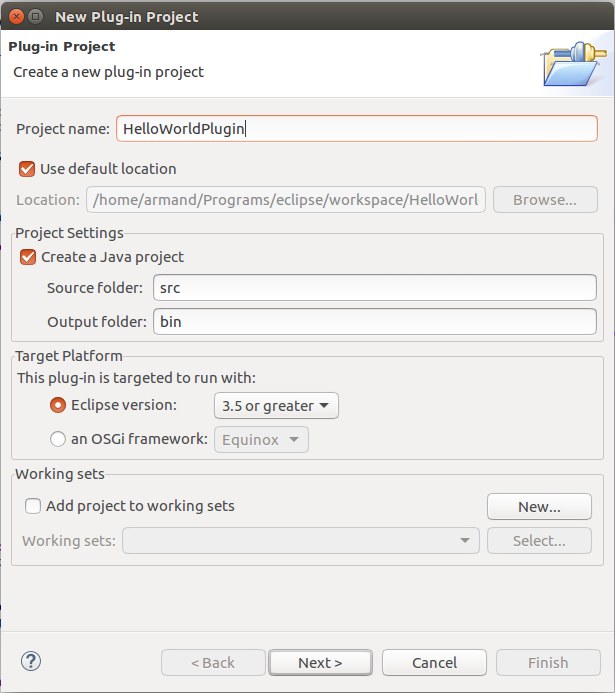
\includegraphics[width=0.4\linewidth]{pictures/newPlugin1.png}\label{fig:newPlugin1}}}%
    \qquad
\subfloat[Création d'un nouveau plugin - 2/4]{{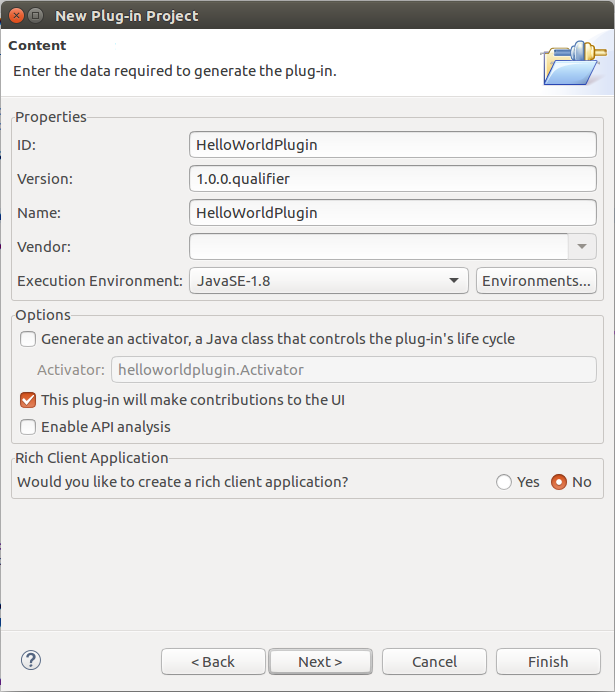
\includegraphics[width=0.4\linewidth]{pictures/newPlugin2.png}\label{fig:newPlugin2}}}%
    \vspace{0.5cm}
\subfloat[Création d'un nouveau plugin - 3/4]{{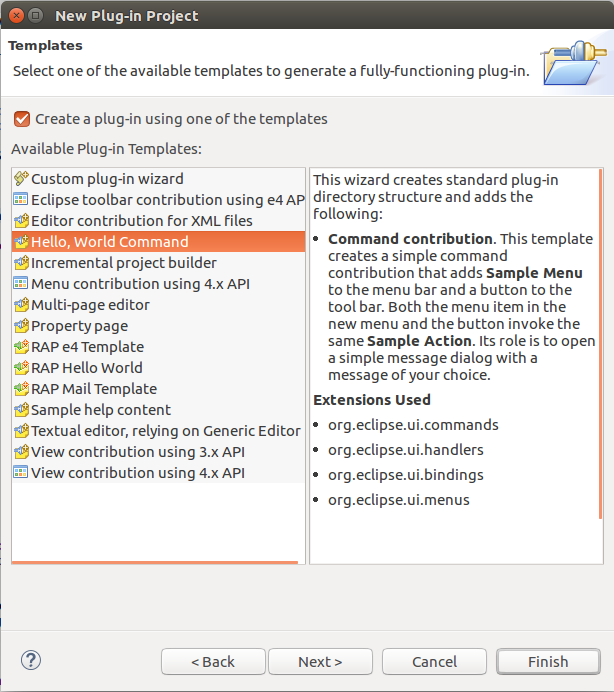
\includegraphics[width=0.4\linewidth]{pictures/newPlugin3.png}\label{fig:newPlugin3}}}%
    \qquad
\subfloat[Création d'un nouveau plugin - 4/4]{{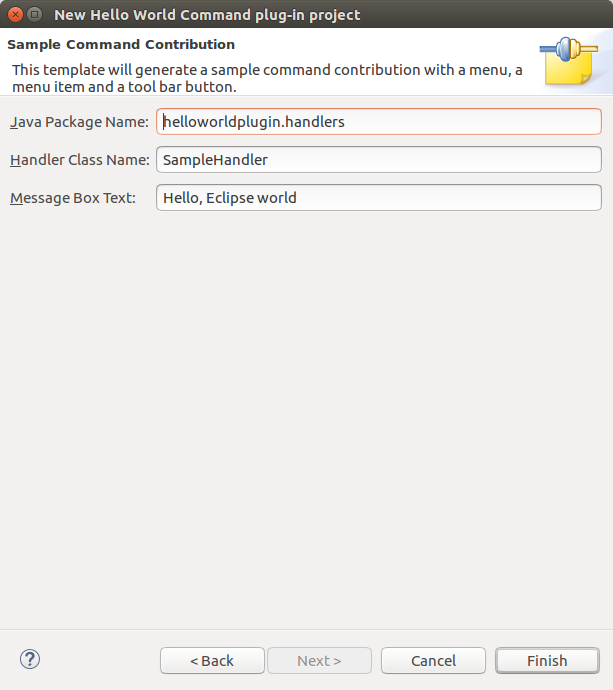
\includegraphics[width=0.4\linewidth]{pictures/newPlugin4.png}\label{fig:newPlugin4}}}%

\caption{Création d'un nouveau plugin dans Eclipse}
\end{figure}


La classe qui nous intéresse est \imtaInlinecode{java}{SampleHandler}, se trouvant dans \imtaInlinecode{text}{./src/helloworldplugin.handlers}.

\begin{imtaCode}{java}
public class SampleHandler extends AbstractHandler {

    @Override
    public Object execute(ExecutionEvent event) throws ExecutionException {
        IWorkbenchWindow window = HandlerUtil.getActiveWorkbenchWindowChecked(event);
            MessageDialog.openInformation(
                            window.getShell(),
                            "HelloWorldPlugin",
                            "Hello, Eclipse world");
            return null;
    }
}
\end{imtaCode}

Nous exécutons le plugin \textit{via} le menu \textit{Run > Run Configurations...}, où nous choisissons \textit{Eclipse Application}, sélectionnons \textit{org.eclipse.platform.ide} %
dans l'encadré \textit{Program to Run} sous l'option \textit{Run a product} (figure \ref{fig:runPlugin1}).
Enfin, nous cliquons sur \textit{Run}.
Une nouvelle instance d'Eclipse s'ouvre, avec un bouton supplémentaire correspondant à notre plugin.
Lorsque nous cliquons sur celui-ci, une fenêtre s'ouvre, affichant le message \textit{"Hello, Eclipse world"} (figure \ref{fig:runPlugin2}).

\begin{figure}[H]
    \centering

    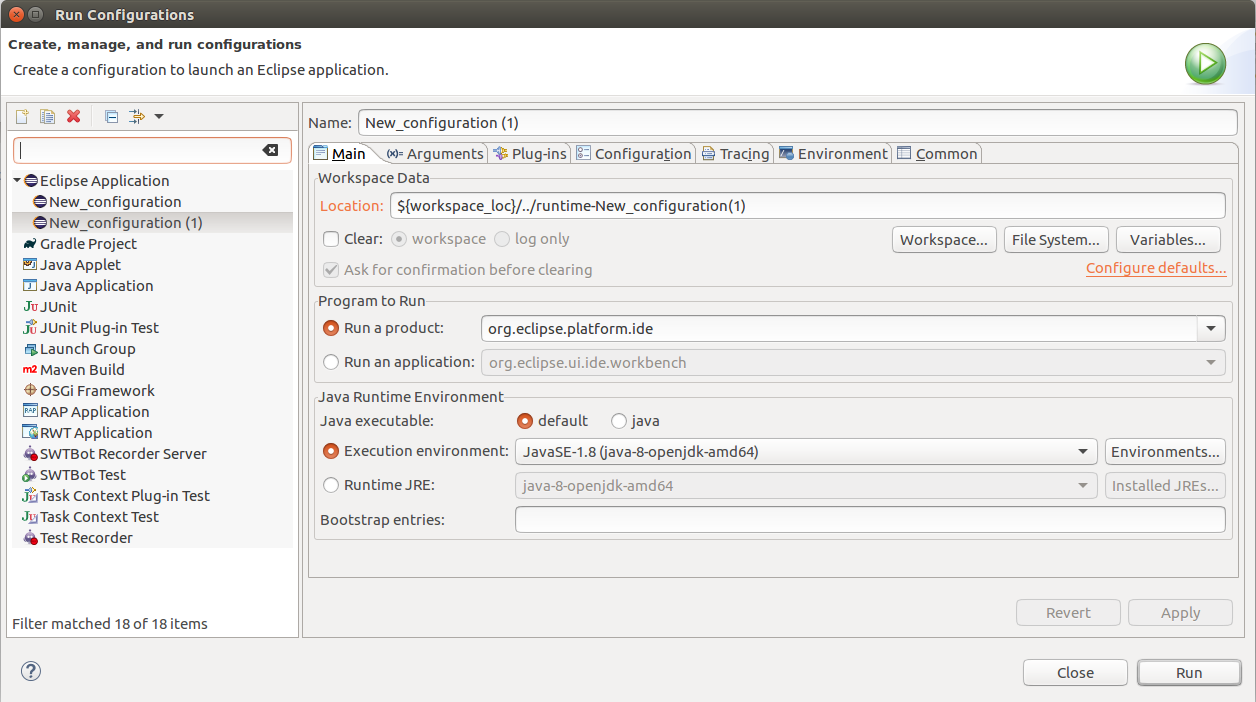
\includegraphics{pictures/runPlugin1.png}

    \caption{Exécution du plugin dans une nouvelle instance d'Eclipse - 1/2}
    \label{fig:runPlugin1}
\end{figure}

\begin{figure}[H]
    \centering

    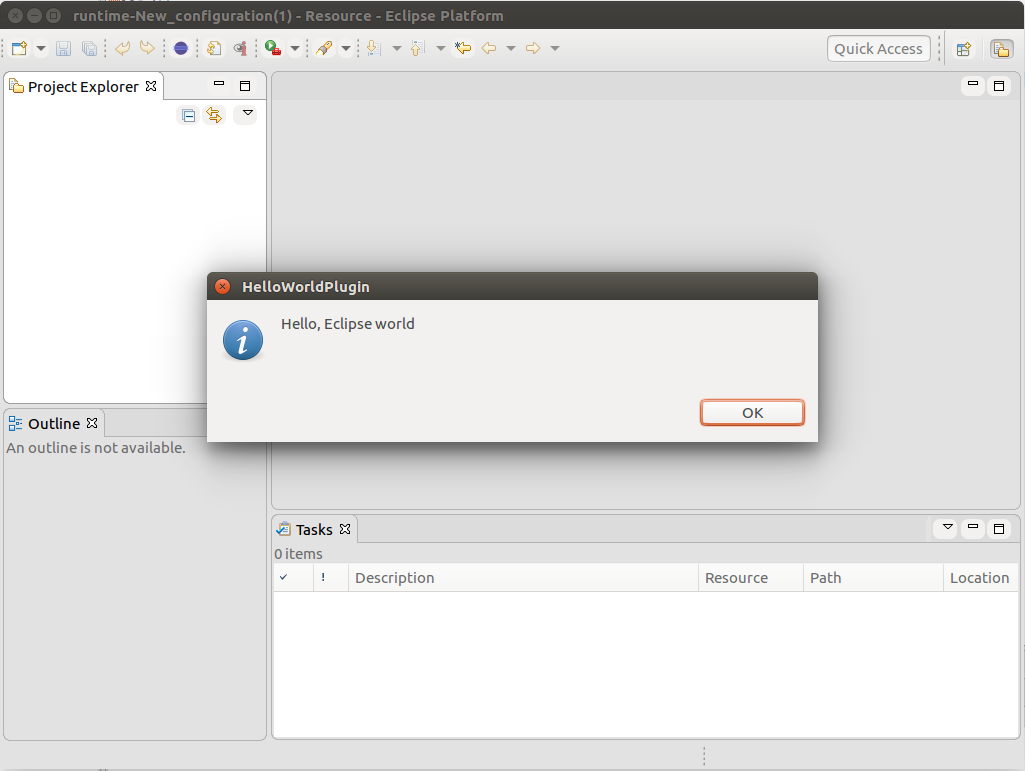
\includegraphics{pictures/runPlugin3.png}

    \caption{Exécution du plugin dans une nouvelle instance d'Eclipse - 2/2}
    \label{fig:runPlugin2}
\end{figure}


\subsection{Intégration dans Rodin}

Nous nous intéressons maintenant à l'intégration du plugin dans Rodin.
Nous téléchargeons tout d'abord Rodin\footnote{%
L'adresse du téléchargement est disponible sur le wiki Rodin : \href{http://wiki.event-b.org/index.php/Main\_Page}{http://wiki.event-b.org/index.php/Main\_Page}}.
Une fois Rodin installé, nous retournons dans notre éditeur Eclipse pour RCP, et choisissons Rodin comme plateforme d'exécution.
Dans le menu \textit{Run > Run Configurations...}, nous choisissons cette fois-ci \textit{org.rodinp.platform.product} comme produit à exécuter, %
puis cliquons sur \textit{Run} (figure \ref{fig:runPlugin3}).
Une instance de Rodin se lance alors, où nous pouvons créer une machine et interagir avec divers composants du monde Event-B, mais aussi %
invoquer notre plugin (figure \ref{fig:runPlugin4}).

\begin{figure}[H]
    \centering

    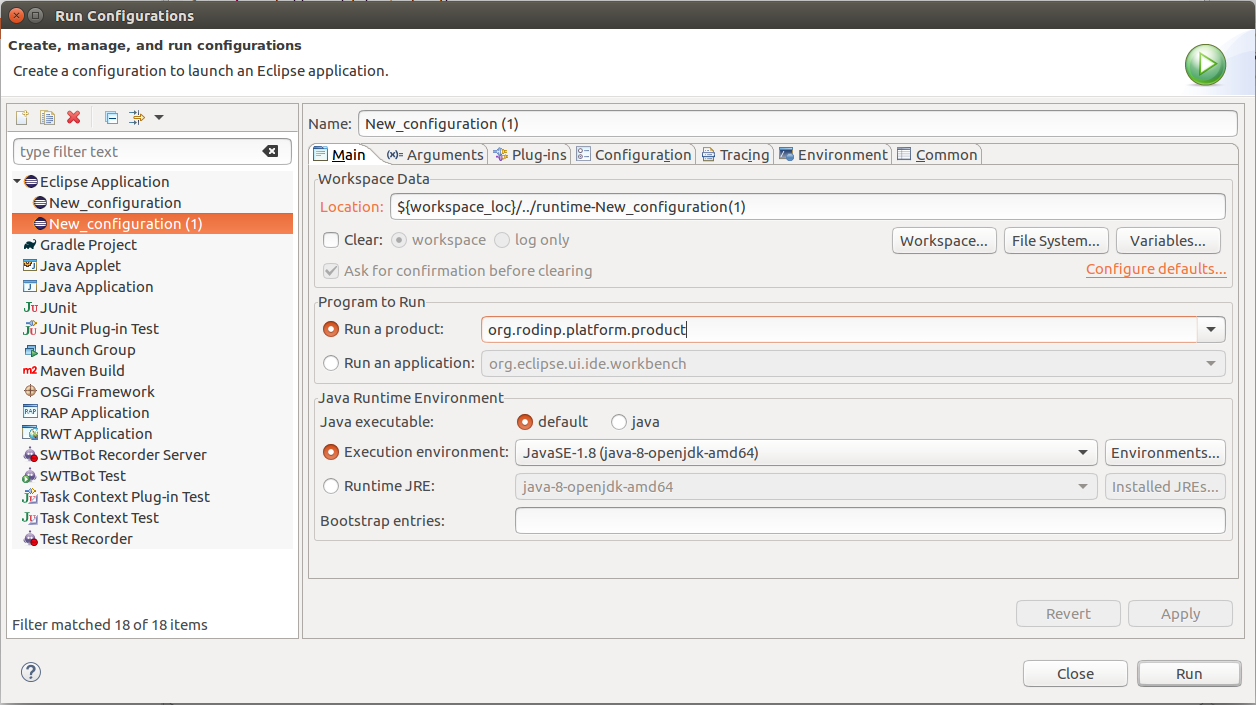
\includegraphics{pictures/runPlugin4.png}

    \caption{Exécution du plugin dans Rodin - 1/2}
    \label{fig:runPlugin3}
\end{figure}

\begin{figure}[H]
    \centering

    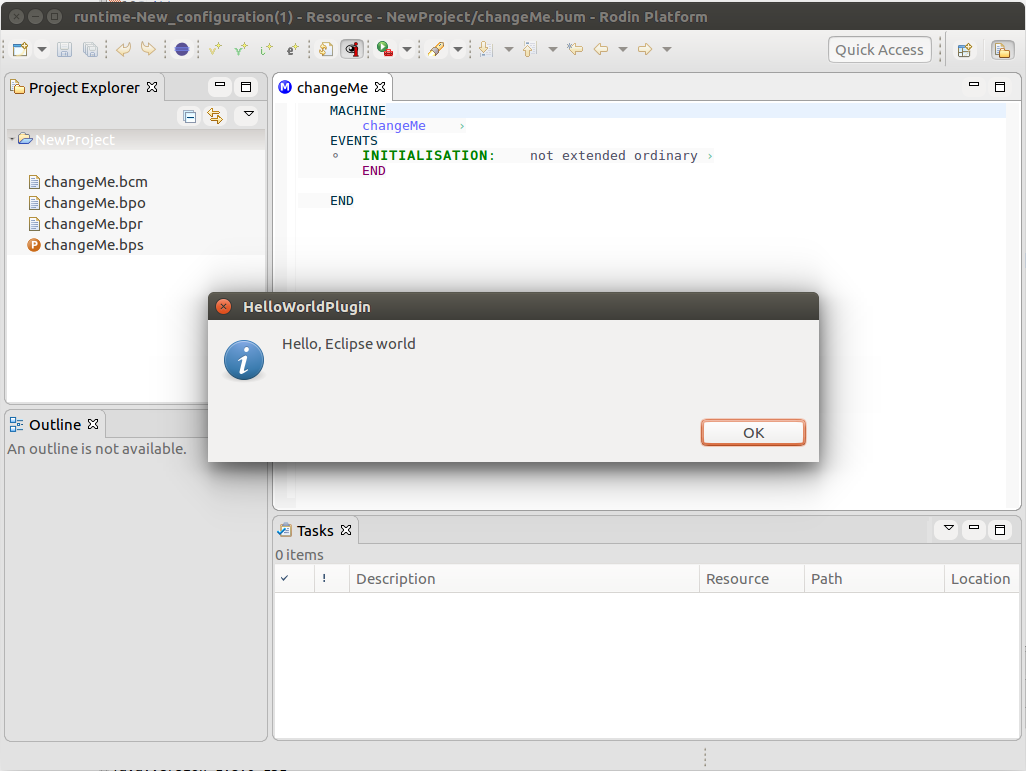
\includegraphics{pictures/runPlugin5.png}

    \caption{Exécution du plugin dans Rodin - 2/2}
    \label{fig:runPlugin4}
\end{figure}


\subsection{Appels à l'API de Rodin}

Nous souhaitons maintenant que notre plugin interagisse avec l'API de Rodin.
Nous ajoutons d'abord les packages nécessaires au manifeste, à savoir \imtaInlinecode{java}{org.eventb.core} et \imtaInlinecode{java}{org.rodinp.core}.
Nous ajoutons également \imtaInlinecode{java}{org.eclipse.core.runtime}, qui contient la classe \imtaInlinecode{java}{CoreException} dont hérite %
\imtaInlinecode{java}{RodinDBException}, levée par la plupart des méthodes utilisées, et qui doit être déclarée pour être attrapée.
Nous ouvrons donc le manifeste comme auparavant, cliquons sur l'onglet \textit{Dependencies}, et cliquons sur le bouton \textit{Add...}.
Nous obtenons une vue semblable à la figure \ref{fig:addDependencies1}, et après validation, l'encadré de dépendances comporte les packages indiqués en figure %
\ref{fig:addDependencies2}.

\begin{figure}[H]
    \centering

    \includegraphics{pictures/addDependencies1.png}

    \caption{Ajout des dépendances au manifeste}
    \label{fig:addDependencies1}
\end{figure}

\begin{figure}[H]
    \centering

    \fcolorbox{gray!50}{white}{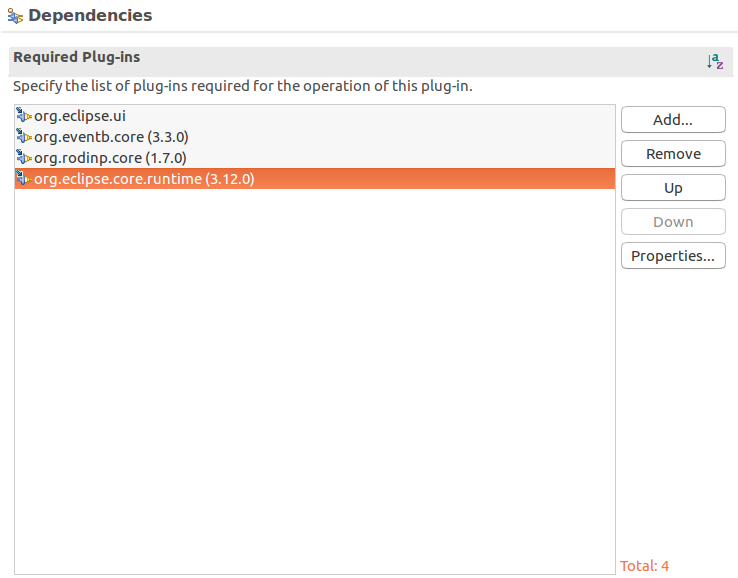
\includegraphics[width=0.6\linewidth]{pictures/addDependencies2.png}}

    \caption{Encadré des dépendances après import}
    \label{fig:addDependencies2}
\end{figure}

Nous créons dans la classe \imtaInlinecode{java}{SampleHandler} une méthode \imtaInlinecode{java}{listProjectElements}, listant les éléments d'un projet dont le nom %
est passé en paramètre.

\begin{imtaCode}{java}
public void listProjectElements(String projectName)
{
    IRodinProject project = RodinCore.getRodinDB().getRodinProject(projectName);
        try
        {
            for (IRodinElement element : project.getChildren())
            {
                if (element instanceof IRodinFile)
                {
                    IInternalElement root = ((IRodinFile) element).getRoot();
                    if (root instanceof IMachineRoot)
                    {
                        for (IInvariant invariant : 
                             ((IMachineRoot) root).getInvariants())
                        {
                            if (invariant.isTheorem())
                            {
                                System.out.println(
                                    "Théorème : " + invariant.getLabel() + " : "
                                    + invariant.getPredicateString());
                            }
                            else
                            {
                                System.out.println(
                                    "Invariant : " + invariant.getLabel() + " : "
                                    + invariant.getPredicateString());
                            }
                        }
                        for (IEvent event : ((IMachineRoot) root).getEvents())
                        {
                            System.out.println("Événement : " + event.getLabel());
                            for (IGuard garde : event.getGuards())
                            {
                                System.out.println(
                                    "Garde : " + garde.getLabel() + " : " 
                                    + garde.getPredicateString());
                            }
                        }
                    }
                }
            }
        } catch (RodinDBException e) {
        e.printStackTrace();
    }
}
\end{imtaCode}

Nous ajoutons un appel à cette méthode dans la méthode principale \imtaInlinecode{java}{SampleHandler.execute}, sur un projet Rodin nommé \imtaInlinecode{java}{"TestProject"}, %
que nous créons et remplissons d'éléments de test, comme en figure \ref{fig:rodinTestProject}.
Enfin, dans la console de l'instance de développement d'Eclipse, nous lisons les éléments listés comme montré en figure \ref{fig:rodinPluginConsole}.

\begin{figure}[H]
    \centering

    \begin{minipage}{.4\linewidth}
        \fbox{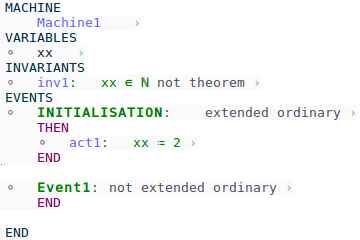
\includegraphics{pictures/rodinTestProject.png}}
        \caption{Machine de test dans Rodin}
        \label{fig:rodinTestProject}
    \end{minipage}%
    \qquad\qquad%
    \begin{minipage}{.4\linewidth}
        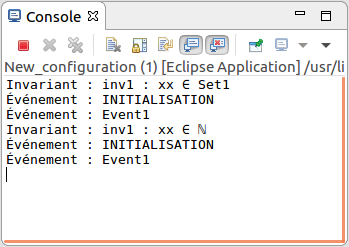
\includegraphics{pictures/rodinPluginConsole.png}
        \caption{Sortie dans la console d'Eclipse}
        \label{fig:rodinPluginConsole}
    \end{minipage}
\end{figure}

Nous pouvons pousser le développement du plugin de test, afin d'afficher les informations précédentes directement dans Rodin, c'est-à-dire dans l'environnement cible.
En reprenant la fenêtre de démonstration du plugin \textit{Hello, World}, nous obtenons la vue présentée en figure \ref{fig:rodinPluginWindow}.

\begin{figure}[H]
    \centering
    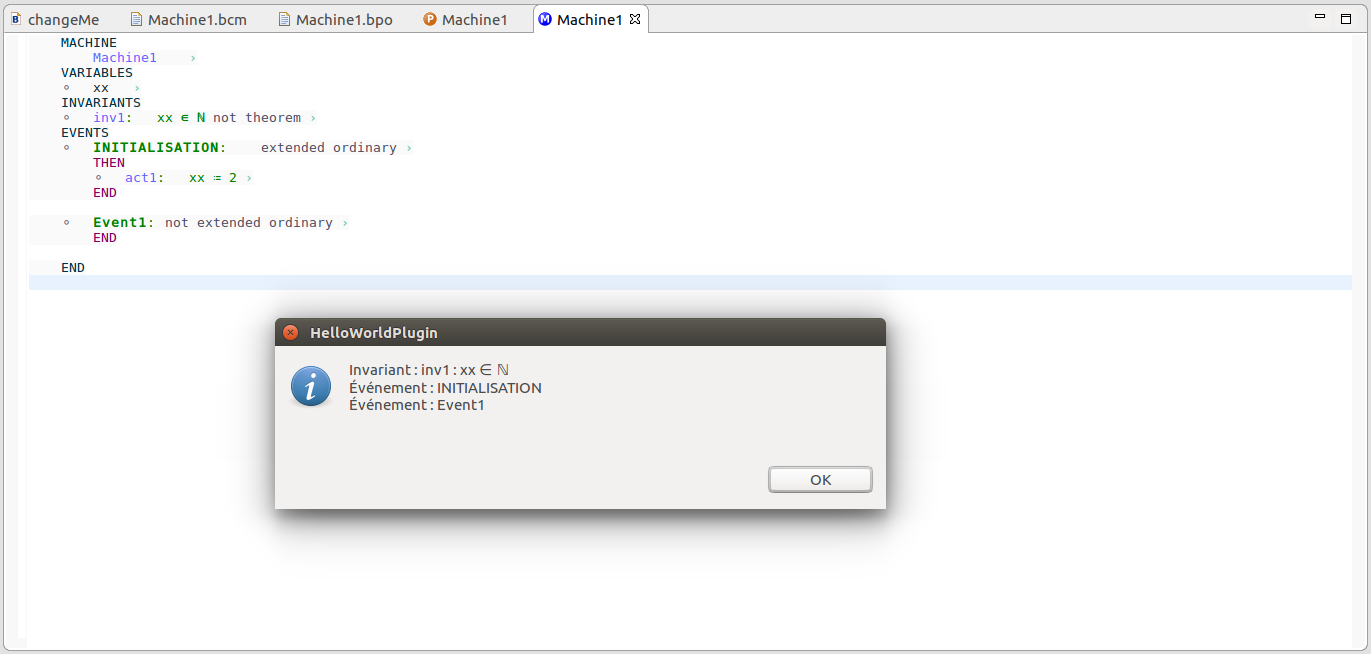
\includegraphics{pictures/rodinPluginWindow.png}
    \caption{Vue de Rodin avec la fenêtre d'informations du plugin}
    \label{fig:rodinPluginWindow}
\end{figure}

Maintenant que nous disposons d'un plugin de base, nous pouvons revenir à notre projet \textit{BlangFlexo} pour implémenter le package \javacode{org.blangflexo.plugin}, afin %
de réaliser la communication désirée.


\section{Communiquer avec OpenFlexo~: le package \texttt{org.blangflexo.plugin}}

% TODO: expliquer rapidement

\subsection{Point d'entrée du plugin}

L'exécution du plugin commence au moment où l'utilisateur appuie sur le bouton ajouté à la barre d'outils de Rodin.
Le \textit{handler} principal du plugin a pour seule fonction de démarrer l'écoute d'instructions, à travers la classe \javacode{InstructionListener} que nous présentons à la section suivante.

\begin{imtaCode}{java}
public class BlangFlexoHandler extends AbstractHandler {
    
    
    @Override
    public Object execute(ExecutionEvent event) throws ExecutionException {
        if (!ApiAbstractor.isStarted())
        	ApiAbstractor.start();
        
        new InstructionListener(20001).start();
        return null;
    }
}
\end{imtaCode}

\subsection{Implémentation d'un serveur TCP}

Nous souhaitons que notre plugin écoute sur une socket TCP les instructions envoyées par OpenFlexo.
Nous implémentons donc un serveur TCP, et OpenFlexo lui enverra ses commandes en mode client.

Le serveur TCP est implémenté par la classe \javacode{org.blangflexo.plugin.InstructionListener}.
Son fonctionnement est volontairement simple~: il attend une connexion sur le port \texttt{20001}, et une fois une connexion acceptée, attend une instruction et l'exécute.
Il renvoie enfin un message indiquant si l'instruction s'est exécutée correctement.

Le serveur est implémenté sous la forme d'un thread, afin de ne pas interférer avec le thread principal d'Eclipse.
Son cycle de vie est implémenté par la méthode \javacode{InstructionListener.run} que nous présentons ici.
La gestion des erreurs et de la fermeture propre de la socket a volontairement été cachée dans le code qui suit pour des raisons de lisibilité, mais est naturellement %
présente dans le code.

\begin{imtaCode}{java}
public void run() {
    String instruction;
    String response;
    ServerSocket socket;
    BufferedReader inFromClient;
    DataOutputStream outToClient;
    
    // Ouverture de la socket d'écoute sur 'port', attribut d'instance
    socket = new ServerSocket(port);
    
    // Acceptation de la connexion cliente
    Socket connectionSocket = socket.accept();
    
    // Création des canaux de communication
    inFromClient = new BufferedReader(new InputStreamReader(connectionSocket.getInputStream()));
    outToClient = new DataOutputStream(connectionSocket.getOutputStream());
    
    // REPL
    while (true) {
        instruction = inFromClient.readLine();
        boolean success = ApiOperationDispatcher.execute(instruction);
        response = success ? "Success" : "Failure";
        outToClient.writeBytes(response);
    }
}
\end{imtaCode}

Les messages reçus par le serveur sont transmis à la classe \javacode{ApiOperationDispatcher}, qui se charge de les interpréter en tant qu'instructions, et de les exécuter.

\subsection{Exécution des instructions}

\newpage
\chapter{Abstraction de l'API Rodin}

Nous souhaitons abstraire les fonctionnalités de gestion de projet de l'API Rodin, afin de fournir une surcouche simple d'utilisation.
Faisant écho aux scénarios de validation, nous présentons d'abord les fonctions abstraites que nous voulons pouvoir appeler sur cette surcouche.


\section{Aperçu de la surcouche}

Nous nous proposons de créer une classe \imtaInlinecode{java}{RodinApiHandle}, qui va proposer les différentes fonctions de la surcouche.
Cette classe présentera l'interface suivante :

% \begin{table}[H]
%     \centering
%     \begin{tabular}{| l | l | l |}
%         \hline
%         \multicolumn{1}{|c|}{Modificateurs} & \multicolumn{1}{|c|}{Signature} & \multicolumn{1}{|c|}{Description}\\
%         \hline\hline
%         \texttt{public static} & \texttt{IRodinProject createRodinProject(final String name)} & Création d'un projet Rodin\\
%         \hline
%         \texttt{public static} & \texttt{IRodinProject createEventbMachine(IRodinProject, final String name)} & Création d'une machine Event-B dans un projet\\
%         \hline
%     \end{tabular}
%     \caption{Interface externe de la surcouche Rodin}
%     \label{table:rodinApiHandle}
% \end{table}

\vspace{\baselineskip}
\begin{labeling}{public static}
    \setlength{\itemsep}{1.5em}

    \item [\javacode{public static}] \javacode{IRodinProject createRodinProject(final String name)}
        \begin{itemize}[label={}]
            \item Création d'un projet Rodin avec le nom donné.
            \item \textit{Dépend de :}
                \begin{itemize}
                    \item \javacode{org.eclipse.core.resources.IWorkspace}
                    \item \javacode{org.eclipse.core.resources.IProject}
                    \item \javacode{org.rodinp.core.IRodinProject}
                \end{itemize}
        \end{itemize}

    \item [\javacode{public static}] \javacode{IMachineRoot createEventbMachine(IRodinProject project, final String name)}
        \begin{itemize}[label={}]
            \item Création d'une machine Event-B dans le projet donné et avec le nom donné.
            \item \textit{Dépend de :}
                \begin{itemize}
                    \item \javacode{org.rodinp.core.IRodinProject}
                    \item \javacode{org.rodinp.core.IRodinFile}
                \end{itemize}
        \end{itemize}

\end{labeling}


\section{Défis de conception}

La conception d'une surcouche à Rodin n'est pas une entreprise si simple qu'il n'y paraît.
D'une part, l'abstraction des fonctionnalités nécessite une compréhension profonde de l'API, et une certaine rigueur vis-à-vis de la validation %
des opérations effectuées.
Par ailleurs, Rodin étant fondé sur Eclipse, il s'avère particulièrement difficile d'extraire son cœur.


\subsection{Validation des opérations réalisées}


\subsection{Extraction du cœur de Rodin}

Au sein de l'API de Rodin, l'implémentation de la méthode Event-B, est contenue dans les packages préfixés par \javacode{org.eventb.}.
La couche de gestion de projet et l'interface utilisateur, quant à elles, sont contenues dans les packages \javacode{org.rodinp.}.
Nous appelons la première région le cœur de Rodin, et la seconde, la couche externe.

La séparation entre ces deux régions est très floue.
Notamment, comme nous l'avons vu en section \ref{sec:rodinApiSummaryEvent}, les classes implémentant les éléments Event-B sont définies dans le cœur de Rodin, %
héritent de \javacode{EventBElement} qui appartient au cœur, mais étendent également \javacode{InternalElement} qui se situe dans la couche externe de l'API.
L'enjeu de cette abstraction est donc avant tout d'isoler les opérations de manipulation de projets et d'éléments.

Toutefois, la manipulation d'un projet Rodin implique une communication avec la base de données Rodin.
Or, celle-ci ne peut être acquise qu'à travers un \textit{workspace}, typiquement de la manière suivante~:

\begin{figure}[H]
\centering
\begin{imtaCode}{java}
final IWorkspace workspace = ResourcesPlugin.getWorkspace();
final IRodinDB rodinDB = RodinCore.valueOf(workspace.getRoot());
\end{imtaCode}
\caption{Acquisition de la base de données Rodin}
\label{fig:rodinDbAccess}
\end{figure}

Nous comprenons qu'un \textit{workspace} doit exister, et que le plugin \javacode{ResourcesPlugin} doit avoir été initialisé.
L'obstacle qui se dessine est précisément la nécessité de l'existence d'une instance d'\javacode{IWorkspace}~: en effet, comme l'indique la documentation %
de l'API d'Eclipse \cite{eclipseiworkspace}, cette interface n'a pas vocation à être étendue ni implémentée par les clients.
Concrètement, cela signifie qu'un \textit{workspace} n'est \textit{a priori} pas censé exister hors d'une instance d'Eclipse.
Ainsi, faire fonctionner le cœur de Rodin hors du mode plugin semble entravé par cette contrainte.

La solution idéale consiste à déterminer et à implémenter une méthode d'instanciation dynamique d'un \textit{workspace} Eclipse.
Cela permettrait de produire une bibliothèque de classes fermée et sans dépendances autres qu'à l'API de Rodin et à celle d'Eclipse.
Une telle bibliothèque serait relativement simple à intégrer à OpenFlexo.
Cette solution offrirait par effet de bord une preuve de concept de l'intégration d'une application RCP Eclipse à OpenFlexo.

Une alternative, nettement moins désirable, consisterait à lancer effectivement une instance de Rodin dans laquelle s'exécuterait un plugin, qui communiquerait %
en réseau, par exemple sur une socket Unix, avec l'instance d'OpenFlexo.
Cette solution, bien qu'elle ait le mérite de contourner l'obstacle, est très peu satisfaisante, car elle n'intègre pas à proprement parler Rodin dans l'écosystème OpenFlexo.
Par ailleurs, elle implique l'exécution d'une instance d'Eclipse en plus d'OpenFlexo, et entraîne une consommation peu utile de ressources supplémentaires.


\section{Développement de la surcouche}

% TODO
% On veut implémenter la solution 1

\subsection{Ouverture du \textit{workspace}}

Afin de pouvoir manipuler des projets Rodin et leurs éléments, il est primordial de disposer d'un \textit{workspace} ouvert.
Il faut donc trouver dans la base de code d'Eclipse quelle classe implémente l'interface \javacode{IWorkspace}, et déterminer une manière de l'instancier.

Une recherche du mot-clé \textit{workspace} dans le moteur de recherche GrepCode\footnote{%
\url{http://grepcode.com/search?query=workspace&start=0&entity=type&n=}} %
permet de trouver la classe \javacode{org.eclipse.core.internal.resources.Workspace}, et d'accéder à son code source \cite{eclipseworkspace}.
Notons au passage que le package \javacode{org.eclipse.core.internal.resources} ne figure pas sur la vue globale des packages de l'API Eclipse \cite{eclipseapioverview}.
Nous essayons donc d'instancier la classe \javacode{Workspace}, avec le code minimal suivant~:

\begin{imtaCode}{java}
import org.eclipse.core.internal.resources.Workspace;    

public class Main {
    public static void main(String[] args) {
        Workspace workspace = new Workspace();
    }
}
\end{imtaCode}

L'exécution de cette classe conduit malheureusement à une exception \javacode{ExceptionInInitializerError}, avec la trace suivante :

\begin{imtaConsole}
Exception in thread "main" java.lang.ExceptionInInitializerError
	at Test.Main.main(Main.java:6)
Caused by: java.lang.NullPointerException
	at org.eclipse.core.internal.runtime.InternalPlatform.getOS(InternalPlatform.java:395)
	at org.eclipse.core.runtime.Platform.getOS(Platform.java:1126)
	at org.eclipse.core.internal.resources.Workspace.<clinit>(Workspace.java:84)
	... 1 more
\end{imtaConsole}

Cette trace nous informe qu'un appel à la méthode statique \javacode{Platform.getOS} a été effectué, mais à échoué lors d'un appel à la méthode d'instance %
\javacode{InternalPlatform.getOS}.
Nous souhaitons investiguer pour trouver la source de l'erreur \javacode{NullPointerException}.


\subsubsection{Analyse du \textit{bytecode} de \texttt{Platform.getOS}}

Ne disposant pas du code source de la classe \javacode{Platform}, nous pouvons malgré tout inspecter le bytecode associé.
Nous trouvons ainsi la définition de la méthode \javacode{getOS}~:

\begin{imtaCode}{java}
// Method descriptor #264 ()Ljava/lang/String;
// Stack: 1, Locals: 0
public static java.lang.String getOS();
  0  invokestatic org.eclipse.core.internal.runtime.InternalPlatform.getDefault() : org.eclipse.core.internal.runtime.InternalPlatform [398]
  3  invokevirtual org.eclipse.core.internal.runtime.InternalPlatform.getOS() : java.lang.String [389]
  6  areturn
    Line numbers:
      [pc: 0, line: 1126]
\end{imtaCode}

La documentation d'Oracle nous renseigne sur le sens des instructions \texttt{invokestatic} \cite{javainvokestatic} et \texttt{invokevirtual} \cite{javainvokevirtual}~: %
la première correspond à l'appel d'une méthode statique, et la seconde à l'appel d'une méthode d'instance.
Nous comprenons donc que la méthode \javacode{Platform.getOS} appelle en premier lieu la méthode statique \javacode{InternalPlatform.getDefault}, %
puis appelle sur l'instance retournée la méthode \javacode{getOS}, et renvoie enfin l'instance de \javacode{String} retournée.
Les appels étant naturellement chaînés façon Java, le code source ressemble probablement à ceci~:

\begin{imtaCode}{java}
public static String getOS() {
    return InternalPlatform.getDefault().getOS();
}
\end{imtaCode}

Si par ailleurs nous essayons d'invoquer la méthode \javacode{InternalPlatform.getDefault}, aucune erreur ne survient.
L'erreur est donc levée à l'intérieur de l'appel à la méthode d'instance \javacode{InternalPlatform.getOS}, comme le laissait entendre la trace d'erreur.


\subsubsection{Analyse du \textit{bytecode} de \texttt{InternalPlatform.getOS}}

Nous nous intéressons maintenant à la méthode d'instance \javacode{InternalPlatform.getOS}, dont le bytecode est le suivant~:

\begin{imtaCode}{java}
// Method descriptor #572 ()Ljava/lang/String;
// Stack: 2, Locals: 1
public java.lang.String getOS();
 0  aload_0 [this]
 1  invokevirtual org.eclipse.core.internal.runtime.InternalPlatform.getBundleContext() : org.osgi.framework.BundleContext [897]
 4  ldc <String "osgi.os"> [18]
 6  invokeinterface org.osgi.framework.BundleContext.getProperty(java.lang.String) : java.lang.String [955] [nargs: 2]
11  areturn
  Line numbers:
    [pc: 0, line: 395]
  Local variable table:
    [pc: 0, pc: 12] local: this index: 0 type: org.eclipse.core.internal.runtime.InternalPlatform
\end{imtaCode}

Comme l'indique la documentation d'Oracle, l'instruction \texttt{aload} \cite{javaaload} pousse une variable sur la pile de la JVM, et l'instruction %
\texttt{ldc} \cite{javaldc} y pousse une valeur scalaire.
Le code source de cette méthode ressemble donc probablement à celui qui suit~:

\begin{imtaCode}{java}
public String getOS() {
    return this.getBundleContext().getProperty("osgi.os");
}
\end{imtaCode}

Nous cherchons la source d'une \javacode{NullPointerException}.
Or, nous savons que \javacode{this} ne pointe pas sur \javacode{null}.


\newpage

\nocite{*}

\printbibheading[title=Références, heading=bibintoc]

\printbibliography[keyword=bmethod, heading=subbibintoc, title={Méthode B}]

\printbibliography[keyword=rodin, heading=subbibintoc, title={Rodin}]

\printbibliography[keyword=openflexo, heading=subbibintoc, title={OpenFlexo}]


\end{document}
%%%%%%%%%% END %%%%%%%%%% 
%%%%%%%%%%%%%%%%%%%%%%%%% 
